\documentclass[11pt]{article}

\newcommand{\yourname}{}
\newcommand{\yourcollaborators}{}

\def\comments{0}

%format and packages%\usepackage{algorithm, algorithmic}
\usepackage{algpseudocode}
\usepackage{amsmath, amssymb, amsthm}
\usepackage{enumerate}
\usepackage{enumitem}
\usepackage{framed}
\usepackage{verbatim}
\usepackage[margin=1.0in]{geometry}
\usepackage{multirow}

\usepackage{microtype}


\usepackage{graphicx}
\usepackage{tikz}
\usetikzlibrary{automata, positioning, arrows.meta}

	\definecolor{processblue}{cmyk}{0.96,0,0,0}


\usepackage{kpfonts}
\usepackage{palatino}
	\DeclareMathAlphabet{\mathtt}{OT1}{cmtt}{m}{n}
	\SetMathAlphabet{\mathtt}{bold}{OT1}{cmtt}{bx}{n}
	\DeclareMathAlphabet{\mathsf}{OT1}{cmss}{m}{n}
	\SetMathAlphabet{\mathsf}{bold}{OT1}{cmss}{bx}{n}
	\renewcommand*\ttdefault{cmtt}
	\renewcommand*\sfdefault{cmss}
	\renewcommand{\baselinestretch}{1.06}
\usepackage{tikz}
	\usetikzlibrary{positioning}
	\definecolor{processblue}{cmyk}{0.96,0,0,0}
    \usetikzlibrary{matrix,arrows}

\tikzset{
->, % makes the edges directed
>=Stealth, % makes the arrow heads bold
node distance=3cm, % specifies the minimum distance between two nodes. Change if necessary.
every state/.style={thick, fill=gray!10}, % sets the properties for each ’state’ node
initial text=$ $, % sets the text that appears on the start arrow
}
	
\usepackage{hyperref}

\hypersetup{
	linktocpage=true,
	colorlinks=true,				% false: boxed links; true: colored links
	linkcolor=blue,		% color of internal links
	citecolor=blue,	% color of links to bibliography
	urlcolor=blue,		% color of external links
}

\usepackage[boxruled,vlined,nofillcomment]{algorithm2e}
	\SetKwProg{Fn}{Function}{\string:}{}
	\SetKwFor{While}{While}{}{}
	\SetKwFor{For}{For}{}{}
	\SetKwIF{If}{ElseIf}{Else}{If}{:}{ElseIf}{Else}{:}
	\SetKw{Return}{Return}

%enclosure macros
\newcommand{\paren}[1]{\ensuremath{\left( {#1} \right)}}
\newcommand{\bracket}[1]{\ensuremath{\left\{ {#1} \right\}}}
\renewcommand{\sb}[1]{\ensuremath{\left[ {#1} \right\]}}
\newcommand{\ab}[1]{\ensuremath{\left\langle {#1} \right\rangle}}

%probability macros
\newcommand{\ex}[2]{{\ifx&#1& \mathbb{E} \else \underset{#1}{\mathbb{E}} \fi \left[#2\right]}}
\newcommand{\pr}[2]{{\ifx&#1& \mathbb{P} \else \underset{#1}{\mathbb{P}} \fi \left[#2\right]}}
\newcommand{\var}[2]{{\ifx&#1& \mathrm{Var} \else \underset{#1}{\mathrm{Var}} \fi \left[#2\right]}}

%useful CS macros
\newcommand{\poly}{\mathrm{poly}}
\newcommand{\polylog}{\mathrm{polylog}}
\newcommand{\zo}{\{0,1\}}
\newcommand{\pmo}{\{\pm1\}}
\newcommand{\getsr}{\gets_{\mbox{\tiny R}}}
\newcommand{\card}[1]{\left| #1 \right|}
\newcommand{\set}[1]{\left\{#1\right\}}
\newcommand{\negl}{\mathrm{negl}}
\newcommand{\eps}{\varepsilon}
\DeclareMathOperator*{\argmin}{arg\,min}
\DeclareMathOperator*{\argmax}{arg\,max}
\newcommand{\eqand}{\qquad \textrm{and} \qquad}
\newcommand{\ind}[1]{\mathbb{I}\{#1\}}
\newcommand{\sslash}{\ensuremath{\mathbin{/\mkern-3mu/}}}

%mathbb
\newcommand{\N}{\mathbb{N}}
\newcommand{\R}{\mathbb{R}}
\newcommand{\Z}{\mathbb{Z}}
%mathcal
\newcommand{\cA}{\mathcal{A}}
\newcommand{\cB}{\mathcal{B}}
\newcommand{\cC}{\mathcal{C}}
\newcommand{\cD}{\mathcal{D}}
\newcommand{\cE}{\mathcal{E}}
\newcommand{\cF}{\mathcal{F}}
\newcommand{\cL}{\mathcal{L}}
\newcommand{\cM}{\mathcal{M}}
\newcommand{\cO}{\mathcal{O}}
\newcommand{\cP}{\mathcal{P}}
\newcommand{\cQ}{\mathcal{Q}}
\newcommand{\cR}{\mathcal{R}}
\newcommand{\cS}{\mathcal{S}}
\newcommand{\cU}{\mathcal{U}}
\newcommand{\cV}{\mathcal{V}}
\newcommand{\cW}{\mathcal{W}}
\newcommand{\cX}{\mathcal{X}}
\newcommand{\cY}{\mathcal{Y}}
\newcommand{\cZ}{\mathcal{Z}}

\newcommand{\opt}{\textsc{opt}}

%theorem macros
\newtheorem{thm}{Theorem}
\newtheorem{lem}[thm]{Lemma}
\newtheorem{fact}[thm]{Fact}
\newtheorem{clm}[thm]{Claim}
\newtheorem{rem}[thm]{Remark}
\newtheorem{coro}[thm]{Corollary}
\newtheorem{prop}[thm]{Proposition}
\newtheorem{conj}[thm]{Conjecture}

\theoremstyle{definition}
\newtheorem{defn}[thm]{Definition}


\newcommand{\instructor}{Drew van der Poel}
\newcommand{\hwnum}{4}
\newcommand{\hwdue}{Sunday, August 7 at 11:59pm via \href{https://www.gradescope.com/courses/406943}{Gradescope}}

\theoremstyle{theorem}
\newtheorem{prob}{Problem}
\newtheorem{sol}{Solution}

\definecolor{cit}{rgb}{0.05,0.2,0.45} 
\newcommand{\solution}{\medskip\noindent{\color{blue}\textbf{Solution:}}}

\begin{document}
{\Large 
\begin{center}{CS3800: Theory of Computation} --- Summer II '22 --- \instructor \end{center}}
{\large
\vspace{10pt}
\noindent Homework~\hwnum \vspace{2pt}\\
Due~\hwdue}

\bigskip
{\large
\noindent Name: \yourname Steve Liu  \vspace{2pt}\\ Collaborators: Eric Chapelaine, Derek Leung, Ares Do, Jamie Lin \yourcollaborators}

\vspace{15pt}
\begin{itemize}

\item Make sure to put your name on the first page.  If you are using the \LaTeX~template we provided, then you can make sure it appears by filling in the \texttt{yourname} command.

\item This assignment is due~\hwdue.  No late assignments will be accepted.  Make sure to submit something before the deadline.

\item Solutions must be typeset.  If you need to draw any diagrams, you may draw them by hand as long as they are embedded in the PDF.  I recommend using the source file for this assignment to get started.

\item I encourage you to work with your classmates on the homework problems. \emph{If you do collaborate, you must write all solutions by yourself, in your own words.}  Do not submit anything you cannot explain.  Please list all your collaborators in your solution for each problem by filling in the \texttt{yourcollaborators} command.

\item Finding solutions to homework problems on the web, or by asking students not enrolled in the class is strictly forbidden.

\end{itemize}



\newpage

\begin{prob} Turing Machine (\emph{6 points})\end{prob}

Give a Turing machine that \emph{decides} the following language $L = \{ w \in \{A,B\}^* |$ the maximum number 
$ \text{of non-overlapping occurences of substring~} AA \text{~is even}\}$.

For example, $ \epsilon, AB, AAAA, AABBAA$, are all in $L$, while $AA, AAA, AABAABBAABBA$ are not.

You should explicitly specify $\Sigma$ and $\Gamma$, in addition to providing a complete diagram of your Turing machine (with states, transitions, etc.). You should use $q_{acc}$ and $q_{rej}$ as your accept and reject states, respectively. You can assume that the input strings are given on the tape, with blank characters following the end of the string.

Provide commentary on the purpose of each state/transition.

\solution \\

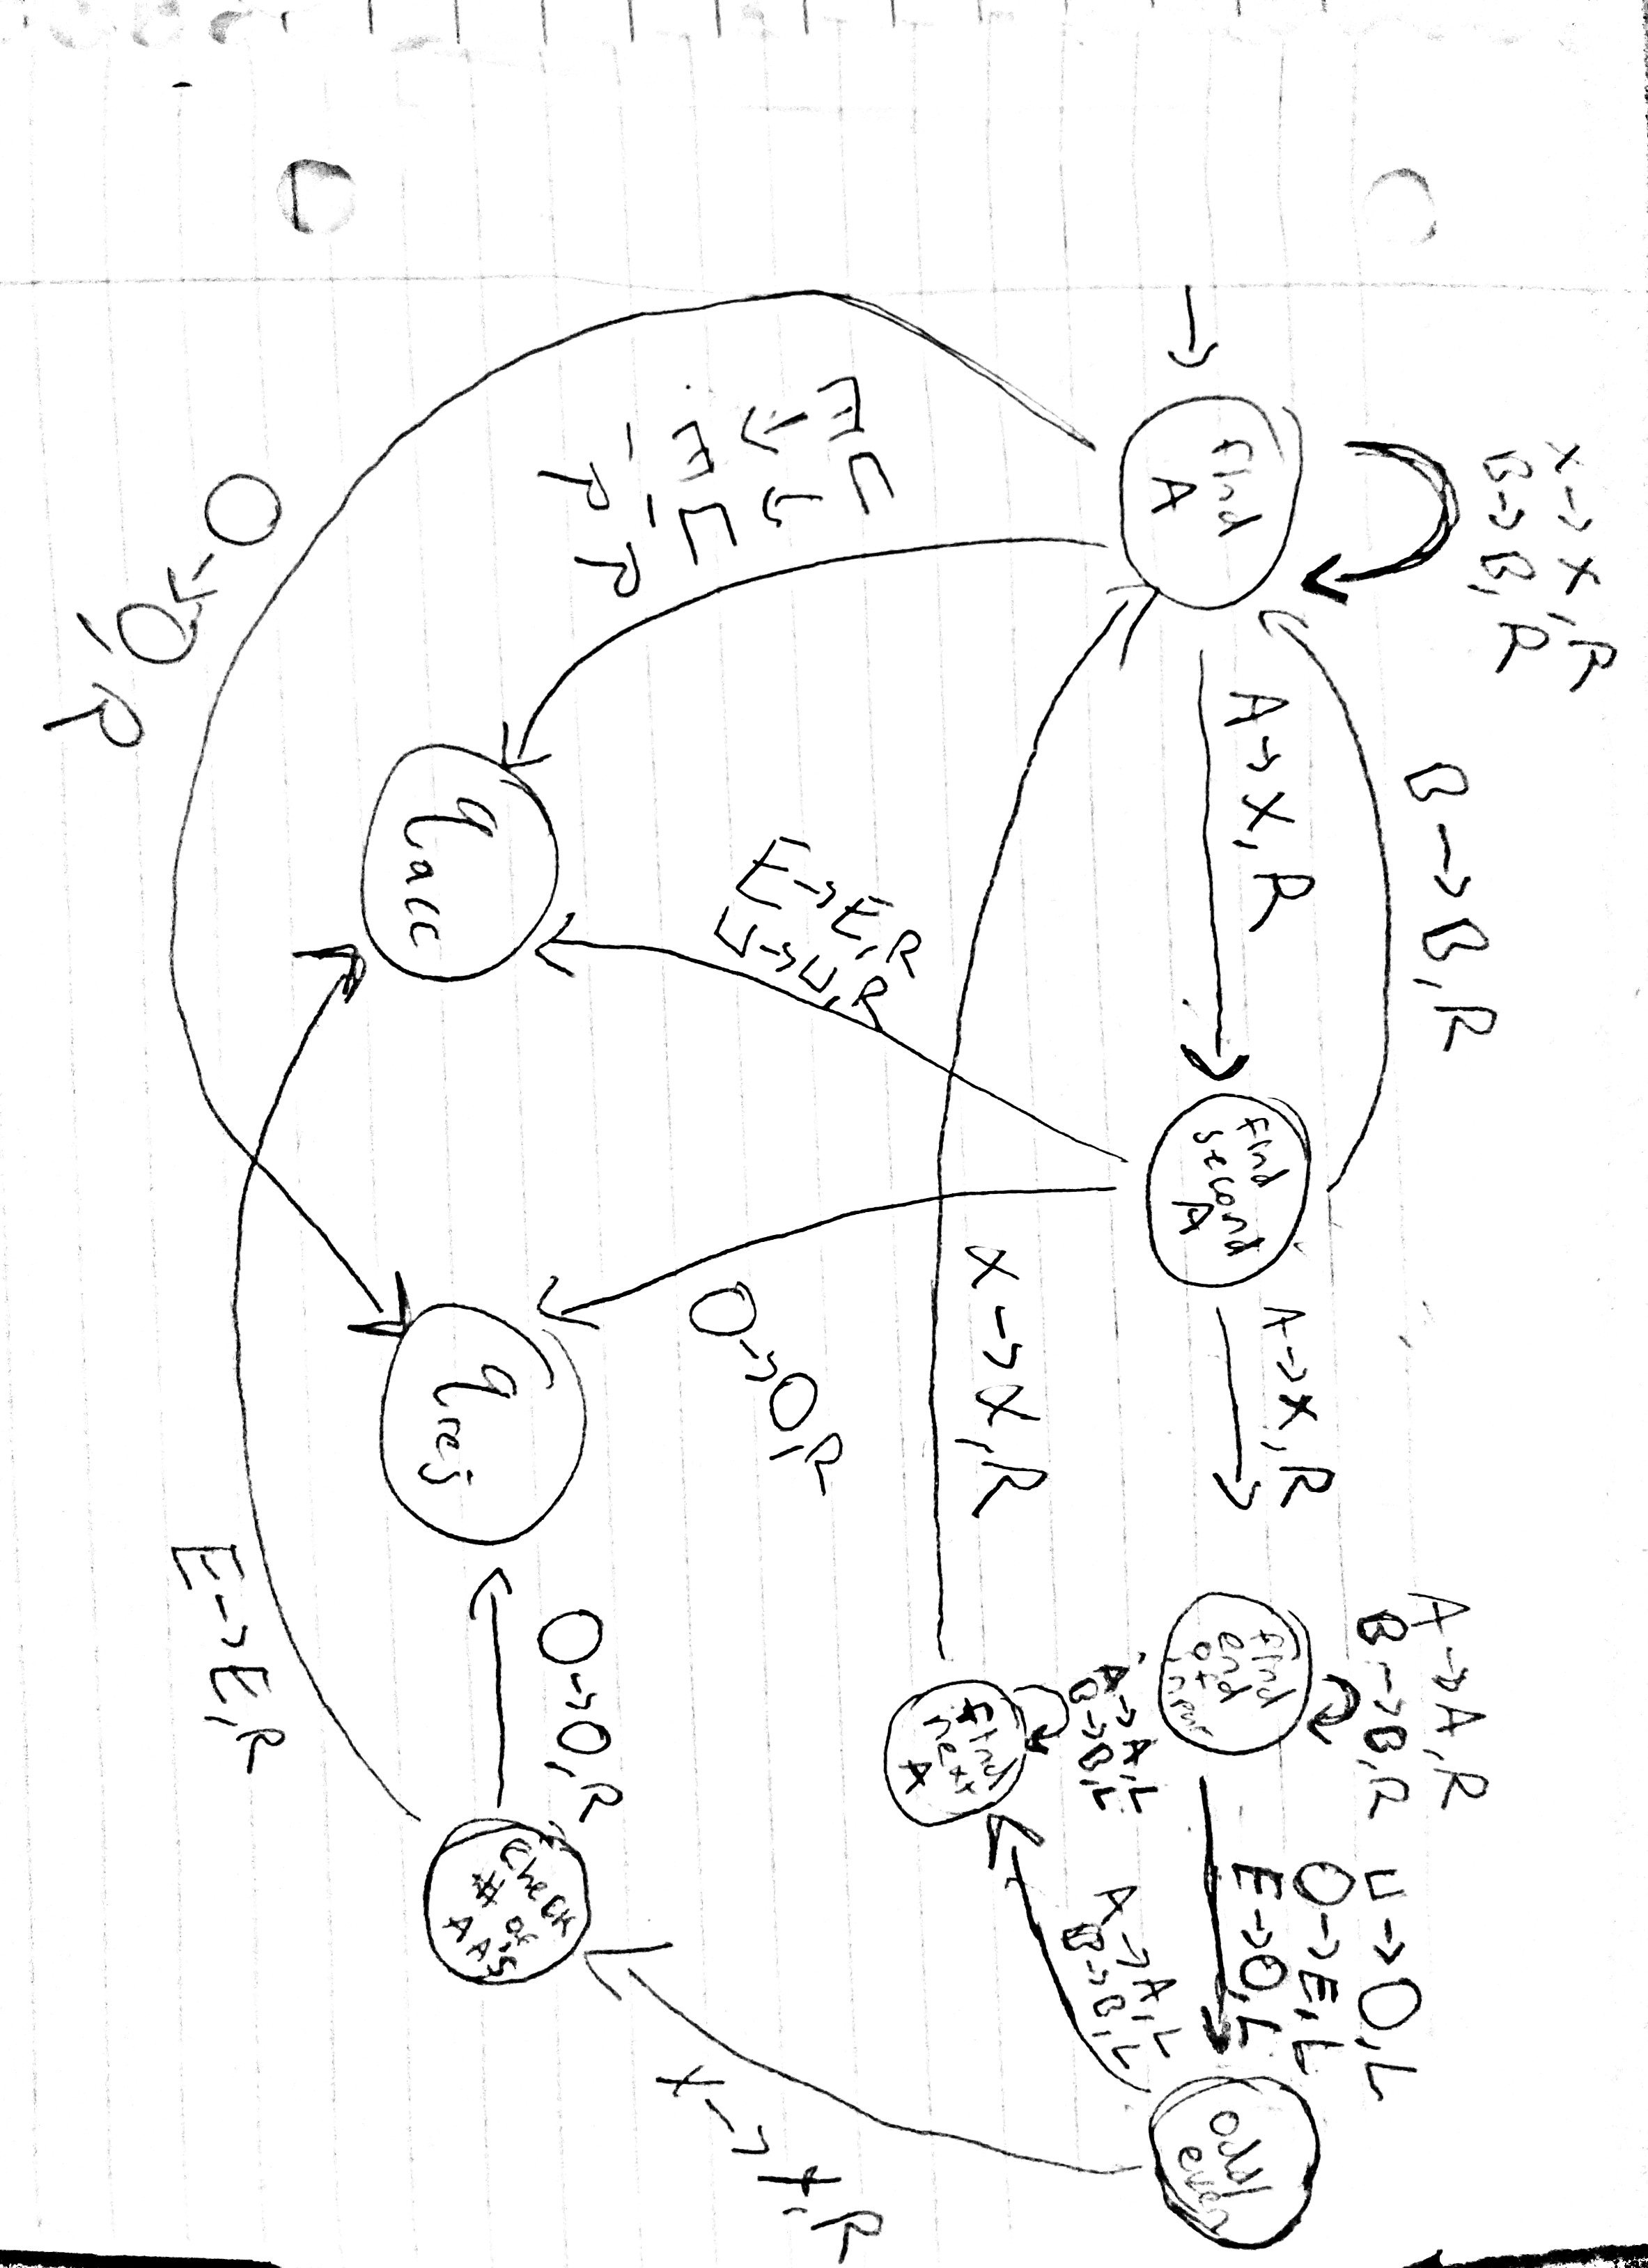
\includegraphics[angle=90,origin=c, scale=0.15]{./hw4p1/hw4p1.jpg}

\noindent$\Sigma$ = $\{A, B \}$ \\
$\Gamma$ = $\{A, B, X, O, E\}$

\newpage
\noindent State: find A \\ 
The purpose of this state is to find the next uncrossed out A by continuously moving to the right on the tape. If we happen to move past the length of the input without finding any uncrossed out A's we can then check on the number of AA's we've found at the end of the input length.
If the value is $\sqcup$ or E then we know that we've found either 0 AA's or an even number of AA's. Otherwise if it's odd then we've found an odd number of AA's \\~\\  

\noindent$\delta$ (find A, A) $\rightarrow$ (find second A, X, R) - We've found the first uncrossed-out A so we want to cross it out and continue to find a second A \\ ~ \\
\noindent$\delta$ (find A, B) $\rightarrow$ (find A, B, R) - Move right on the tape head until we find the first uncrossed out A \\ ~ \\
$\delta$ (find A, X) $\rightarrow$ (find A, X, R) - Move right on the tape head until we find the first uncrossed out A \\ ~ \\
$\delta$ (find A, $\sqcup$) $\rightarrow$ ($q_{acc}$, $\sqcup$, R) - We've reached the end of the input on the tape and we've found 0 AA's \\ ~ \\
$\delta$ (find A, E) $\rightarrow$ ($q_{acc}$, E, R) - We've reached the end of the input on the tape without finding any extra A's and we've found an even number of AA's \\ ~ \\
$\delta$ (find A, O) $\rightarrow$ ($q_{rej}$, O, R) - We've reached the end of the input on the tape without finding any extra A's and we've found an odd number of AA's \\ ~ \\

\noindent State: find second A \\ 
The purpose of this state is to check if we've found a second adjacent A. \\ ~ \\

\noindent$\delta$ (find second A, A) $\rightarrow$ (find end of input, X, R) - We've found a second adjacent A so we want to cross it out and move to the end of the input\\ ~ \\
\noindent$\delta$ (find second A, B) $\rightarrow$ (find A, B, R) - Did not find a second adjacent A so we want to continue finding the next uncrossed out A \\ ~ \\
$\delta$ (find second A, $\sqcup$) $\rightarrow$ ($q_{acc}$, $\sqcup$, R) - We've reached the end of the input on the tape and we've found 0 AA's \\ ~ \\
$\delta$ (find second A, E) $\rightarrow$ ($q_{acc}$, E, R) - We've reached the end of the input on the tape and we've found an even number of AA's \\ ~ \\
$\delta$ (find second A, O) $\rightarrow$ ($q_{rej}$, O, R) - We've reached the end of the input on the tape and we've found an odd number of AA's \\ ~ \\

\noindent State: find end of input \\ 
Traverses to the end of the input string length, and marks whether or not we've seen an even or odd number of AA's. \\ ~ \\
\noindent$\delta$ (find end of input, A) $\rightarrow$ (find end of input, A, R) - Keep moving the tape head right until we've reached the end\\ ~ \\
\noindent$\delta$ (find end of input, B) $\rightarrow$ (find end of input, B, R) - Keep moving the tape head right until we've reached the end\\ ~ \\
$\delta$ (find end of input, $\sqcup$) $\rightarrow$ (alternate odd/even, O, L) - We've reached the end of the input on the tape and we've found only 1 AA's \\ ~ \\
$\delta$ (find end of input, E) $\rightarrow$ (alternate odd/even, O, L) - We've reached the end of the input on the tape and we've found an even number of previously so we want to switch it to odd \\ ~ \\
$\delta$ (find end of input, O) $\rightarrow$ (alternate odd/even, E, L) - We've reached the end of the input on the tape and we've found an odd number of previously so we want to switch it to even \\ ~ \\

\noindent State: alternate odd/even \\
Alternates between E and O symbols to check whether or not we're seen an even or odd number of AA's \\ ~ \\
\noindent$\delta$ (alternate odd/even, A) $\rightarrow$ (find next A, A, L) - After changing the even/odd mark at the end of the string, move left to find the next uncrossed out A\\ ~ \\
\noindent$\delta$ (alternate odd/even, B) $\rightarrow$ (find next A, B, L) - After changing the even/odd mark at the end of the string, move left to find the next uncrossed out A\\ ~ \\
\noindent$\delta$ (alternate odd/even, X) $\rightarrow$ (check $\#$ of AA's, X, R) - If the last value in the input string is an A that has been crossed out, we can then check move to the marked value at the end of the string to check if we've seen an even number of AA's or not\\ ~ \\

\noindent State: find next A \\
Moves tape head left to find the first instance of a crossed out A and resets the algorithm to repeat finding the next uncrossed out A. \\ ~ \\
\noindent$\delta$ (find next A, A) $\rightarrow$ (find next A, A, L) - Moves tape head left to find the first instance of an uncrossed out A\\ ~ \\
\noindent$\delta$ (find next A, B) $\rightarrow$ (find next A, B, L) - Moves tape head left to find the first instance of an uncrossed out A\\ ~ \\
\noindent$\delta$ (find next A, X) $\rightarrow$ (find A, X, R) - We've found a crossed out A so we reset to find the next uncrossed out A\\ ~ \\

\noindent State: check $\#$ of AA's \\
If the last value on the input part of the tape is a crossed out A, we move the tape head to the right and check if we've seen an even number of AA's \\ ~ \\
\noindent$\delta$ (check $\#$ of AA's , E) $\rightarrow$ ($q_{acc}$, O, R) - We've reached the end of the input on the tape and we've found an even number of AA's \\ ~ \\
\noindent$\delta$ (check $\#$ of AA's , O) $\rightarrow$ ($q_{rej}$, E, R) - We've reached the end of the input on the tape and we've found an odd number of AA's \\ ~ \\

\newpage

\begin{prob} Alternate TMs (\emph{2 points})\end{prob}

Consider a new Turing machine that instead of moving one cell left or right, we can only move left 4 cells and right 2 cells. Can this new Turing machine be used in place of the standard Turing machine? That is, can it recognize any language that the standard one can? If yes, provide sound reasoning as to why this is. If not, give an example of a language which cannot be recognized by the new Turing machine, but can be recognized by the standard variant.

Note that the input will still be given consecutively on the tape, it is not spaced out to accommodate the new machine.

\solution \\
No the new Turing machine variant cannot be used in place of the standard Turing machine. An example of language that the new Turing Machine can't recognize but the standard one can is: \\ ~ \\

\noindent $L = $\{$ w | w \in \{0, 1\}$* and there is at least one 0 in $w$ $\}$ \\~\\

\noindent An example of a string that is in $L$ is $101$, however, the new TM won't recognize this string since the head has to move right two cells, so it will skip the 0 in the middle and reject the string. \\ 

\noindent The standard TM would recognize this language since the algorithm involves walking through each symbol in the input one-by-one and finding the first 0. 

\newpage

\begin{prob} True/False: Enumerators (\emph{6 points})\end{prob}


For each of the following assertions, state whether it is true or false, and justify your answer. You do not need prove undecidability. You can assume that the alphabet $\Sigma = \{0, 1\}$ in the following problems.

\begin{enumerate}[label=(\alph*)]

\item \textbf{[2 pts.]} If $E$ is an enumerator, then there exists a TM $D$ which is a decider such that $L(D) = L(E)$.  

\solution \\
False. $E$ can generate Turing-recognizable languages which $D$ cannot recognize which means that $L(D)$ may not be equal to $L(E)$.


\item \textbf{[2 pts.]} If $D$ is a TM which is a decider, then there exists an enumerator $E$ such that $L(E) = L(D)$.


\solution \\
True. All Turing recognizable languages have an enumerator that generates the strings in the language. Therefore since the set of Turing-decidable languages is a subset of Turing-recognizable languages, there exists an enumerator that recognizes the decider, $D$. 




\item \textbf{[2 pts.]} Based on the above results, are deciders and enumerators equally powerful (can they decide/generate the same set of languages)? If yes, why is this the case? If no, which is more powerful and why is that?

\solution \\
No, enumerators are more powerful since they can generate Turing-recognizable languages while deciders can only recognize Turing-decidable languages which are a subset of Turing-recognizable.


\end{enumerate}


\newpage

\begin{prob} Decidable DFA Problems (\emph{16 points})\end{prob}

Consider the following computational problem: Does a given DFA accept any strings of length 5?

\begin{enumerate}[label=(\alph*)]

\item \textbf{[1 pt.]} Give the corresponding language, $L^5_{DFA}$, for this problem.

\solution

$L^5_{DFA}$ = $\{<M> |$ M is a DFA and there exists $w$ in $L(M)$ such that $|w| = 5$ $\}$


\item \textbf{[5 pts.]} Prove that $L^5_{DFA}$ is decidable. You can do this by giving an algorithm, as we did in class. Justify your approach.

\solution
\\
Let $T$ be the Turing Machine on $L^5_{DFA}$. On input $M$: \\ ~ \\
1. Generate all possible valid strings of length 5, let's call this set of strings $L$. \\ ~ \\
2. For each string, $w$ $\in$ $L$, run the Turing Machine, $D_{A-DFA}$, that decides the DFA acceptance problem (we were shown this in class) on input $<M, w>$. \\ ~ \\
3. If $D_{A-DFA}$ ever accepts, then $T$ should accept and if $D_{A-DFA}$ rejects on all of the generated strings, then $T$ should reject. \\ ~ \\


For step 1, by the definition of a $DFA$, the set of input symbols in the alphabet must be finite and we also know that only valid strings of length 5 can be generated.
Because of these two facts, the cardinality of the set of strings of length 5 must be a finite value since there are only so many combinations of strings of length 5 that can be created with a finite alphabet. The cardinality of this set would actually be $|\Sigma|^5$ where $\Sigma$ is $M$'s alphabet. \\ ~ \\
For step 2, $D_{A-DFA}$ is a Turing Machine that decides whether or not a given DFA accepts a given string. Since the set of strings that are we are running through $D_{A-DFA}$ is finite and $D_{A-DFA}$ is a decider, this step must eventually halt. \\ ~ \\
For step 3, if $D_{A-DFA}$ ever accepts then we know that the given DFA $M$ must accept at least one string of length 5 so $T$ would accept. Alternatively, if $D_{A-DFA}$ rejects on all strings then we want to $T$ to reject since there are no strings of length 5 that is accepted.


\item \textbf{[1 pt.]} Now we generalize the problem further; does a given DFA accept any strings of a length which is divisible by 5? Give the corresponding language $D^5_{DFA}$ for this new problem.

\solution


$D^5_{DFA}$ = $\{<M> |$ M is a DFA and there exists $w$ in $L(M)$ such that $|w|$ $\%$ 5 = 0 $\}$




\item \textbf{[5 pts.]} Prove that $D^5_{DFA}$ is decidable. You can do this by giving an algorithm, as we did in class. Justify your approach.

\solution
\\
Let $T_1$ be the Turing Machine on $D^5_{DFA}$. On input $M$: \\ ~ \\ 
1. Generate a set of all valid strings of length 5, let's denote this set as $L$. \\ ~ \\
2. Construct $D_{L^*}$ to be the DFA that recognizes $L$* (which is the set of all strings that have a length of multiple of 5)  \\ ~ \\
3. Construct $D_{INTERSECTION}$ to be the DFA that recognizes $L(M) \cap L(D_{L^*})$ \\ ~ \\
4. Run the Turing Machine, $E_{DFA}$, that decides the DFA emptiness problem (we were shown this in class) on input $<D_{INTERSECTION}>$ \\ ~ \\
5. If $E_{DFA}$ accepts, then $T_1$ rejects and if $E_{DFA}$ rejects then $T_1$ accepts. \\ ~ \\

For step 1, the process of generating all valid strings of length 5 is finite as explained in the earlier problem. \\ ~ \\ 
For step 2, since we know that the set $L$ is a regular language (its Regular Expression would be $\Sigma\Sigma\Sigma\Sigma\Sigma $ where $\Sigma$ is the union of all characters in the alphabet of $M$) and that since regular languages are closed under the star operation, the resulting language $L$* is also a regular language which means it can be recognized by a DFA. Since we know that $L$ is the set of all strings that have a length of 5, then $L$* has to be the set of all strings that are divisible or is a multiple of 5 since appending strings of length 5 together gives you strings of multiples of 5. \\ ~ \\ 
For step 3, intersecting the language recognized by DFA $M$ and DFA $D_{L^*}$ will give you the set of all strings that are recognized by $M$ and has the property of its length being divisible by 5 by the definition of intersection. Furthermore, since we also know that regular languages are closed under intersection, the resulting language is also regular which means that there does exist a DFA that recognizes it. \\ ~ \\
For step 4 + 5, $E_{DFA}$ is a Turing Machine that decides whether or not a given DFA accepts no string, so if we run $E_{DFA}$ on $<D_{INTERSECTION}>$ and $E_{DFA}$ accepts, then we know that the there are no strings in the language recognized by $M$ that satisfies the property of having a length divisible by 5 so we want $T_1$ to reject. Alternatively, if $E_{DFA}$ rejects, then we know there is at least one string in the language recognized by $M$ that does have length divisible 5, so $T_1$ would accept.

\item \textbf{[4 pts.]} Consider generalizing the problem even further; does a given DFA accept any strings of a length which is divisible by a given value $d$? Give the corresponding language for this problem (you can name it whatever you want). Is this language decidable? If yes, state how to modify your algorithm from part (d). If no, argue why not.

\solution
\\
Let $L_{d}$ = $\{<M, d> |$ M is a DFA and there exists $w$ in $L(M)$ such that $|w|$ $\%$ $d$ = 0 $\}$ \\ ~ \\
$L_d$ is decidable and we can modify steps 1 and 2 from the algorithm in part d.\\

Step 1: We will now generate all valid strings of length $d$ rather than length 5 so $L$ will now be a set of all strings that have a length of $d$ \\

Step 2: $L$* will now be the set of all strings that have a length of multiple of $d$. \\ ~ \\

JUSTIFICATION: \\
Modification to step 1: Assuming $d$ is some finite value, the generation of all valid strings of length $d$ is still going to be a finite process for the same reasons stated in the previous parts. \\~\\ 
Modification to step 2: $L$ is still going to be a regular language (its regular expression would just be $d$ number of $\Sigma$'s concatenated together) so if we star it, $L$* will still be another regular language. \\~\\ 

Since the assumptions in the modified algorithm have not really changed, the rest of steps in the algorithm should follow through in the same manner. As a result, $L_{d}$ is a decidable language. 


\end{enumerate}

\end{document}
